% Chapter 8

\begin{savequote}[\quotewidth]
It is a bad plan that admits of no modification.
\qauthor{Publilius Syrus}
\end{savequote}

\chapter{Modified CO\textsubscript{2} as mobile phase for SFC×GC} % Main chapter title
\label{Chapter8}

\section{Introduction}

The previous chapters described SFC×GC runs that used neat carbon dioxide as
mobile phase for the SFC separation. Carbon dioxide as a mobile phase is
compatible with a flame ionization (FID) detector: under the conditions found in
the hydrogen-rich portion of the flame the carbon dioxide cannot be reduced to
methane, the first step in the process that produces the ions that gives the FID
its name. But most modern SFC development involves the use of modifiers and
additives\footnote{Nominally, modifiers are added to the carbon dioxide to
manipulate the solubility of the analytes in the mobile phase, in the same way
that mixtures of solvents are used in, say, gradient elution in HPLC. Additives
are added in small amounts and manipulate the interaction of the analyte with
the stationary phase. In reality, the mechanism of their action is more complex
\autocite{Berger1991}.}. These modifiers are usually organic compounds, and in
the FID flame they produce ions. When the modifier-containing eluate of an SFC
column passes through the detector, the quantity of the modifiers will be much
higher than quantity of the analytes. If the detector is an FID, the modifiers
will produce many more ions than the analyte will produce, and therefore the the
modifier signal will swamp the analyte signal. Mixing organic modifiers and
additives with the carbon dioxide mobile phase therefore renders SFC
incompatible with flame ionization as a detection method. As a result, most
modern SFC chromatographs use optical detectors, most commonly UV
spectrophotometry adopted from HPLC.

While the use of optical detectors has not hampered the development of SFC,
they do have a few shortcomings, which might be imposing artificial limits on
the exploitation of the versatility of carbon dioxide as a mobile phase:

\begin{itemize}

\item While SFC is compatible with optical detection (carbon dioxide does not
absorb visible or ultraviolet radiation), there is a wide range of potential
modifiers that are not compatible with spectrophotometric detection because they
absorb strongly in the UV, but might have chemical properties useful for
manipulating SFC separations. 

\item Optical detectors can only detect analytes with chromophores, and the
intensity of the signal depends strongly on the species.

\item Optical detectors have a limited dynamic range, which complicates
quantification.

\item Expensive 'HPLC-grade' solvents do not provide better chromatography than
other grades of solvents: the processes used to purify them are just optimized to
reduce the amount of UV-absorbing impurities that can interfere with analysis.

\end{itemize}

In comparison, the FID can detect practically any organic compound over a wide
concentration range, giving an integrated-over-time signal proportional to the
mass of the compound.

When GC is comprehensively coupled to SFC, the modulator will focus each
fraction of SFC eluate, and then the GC will separate all the compounds in the
fraction, be they analytes, modifiers, or additives. If the modifiers are more 
volatile than the analytes, the modifiers will elute before the analytes, and
the analyte can be detected or quantified using an FID while the signal from the
modifier is ignored.

Of course it is quite likely that the peak from the modifiers will
\keyword{overload} the GC. Both the detector and the column may be overloaded.
If the \emph{detector} is overloaded, it just means that the detector no
longer responds linearly to the amount of material eluting from the column ---
this might include responding with its maximum output, leaving flat-topped
peaks. If the \emph{column} is overloaded, the capacity of the stationary
phase is exceeded and the peaks will \keyword{front}: they will be asymmetrical,
with the side of the peak towards earlier elution times having a slope smaller
than the slope of non-overloaded peaks, and the side of the peak towards later
elution times having a larger slope.

The requirement that the modifiers added to the SFC mobile phase be volatile (so
that they can elute before the analyte) is not too onerous a restriction. Higher
volatility correlates with higher diffusivity, so that the preferred
high-diffusivity modifiers for SFC  would also tend to be be volatile enough to
elute early on GC. 

A practical SFC×GC chromatograph opens up the field for the use of carbon
dioxide mixed with modifier as a mobile phase for analysing complex mixtures
found in biodiesel production, biodiesel quality control, and compliance
monitoring.

\section[SFC×GC with modifier]{SFC×GC using modified carbon dioxide.}

In this section a SFC×GC chromatogram is presented that shows that methanol
added as a modifier to the SFC mobile phase does not interfere with the fast GC
any more than a sample's solvent interferes in the usual 1D GC. The 2D
separation space of SFC×GC therefore gains in control over elution in the SFC
dimension at the cost of losing the capability to detect compounds more volatile
than methanol on the GC dimension: modifiers can help elute more polar compounds
on SFC, but they will co-elute with volatile analytes and saturate the detector.

\subsection{Sample}

The sample was a 1:1 blend of petrodiesel and biodiesel, prepared in the
laboratory. The biodiesel sample was donated by a commercial testing laboratory
and had been produced from palm oil by an anonymous producer. The petrodiesel
(Shell Extra Diesel 500 ppm) was obtained from a commercial filling station.

\subsection{SFC}

The SFC used carbon dioxide at \SI{200}{\bar} inlet pressure and room
temperature as mobile phase, into which \SI{0.5}{\micro\litre} of sample was
injected. The flow rate of carbon dioxide at atmospheric pressure was
\SI{175}{\milli\litre\per\minute}, corresponding to a mass flow rate of about
\SI{0.3}{\gram\per\minute}. The carbon dioxide mobile phase was modified with
\SI{5}{\percent} mass fraction of HPLC-grade methanol (Merck LiChrosolv).
The column consisted of five HPLC bare silica columns (\SI{150}{\milli\metre}
$\times$ \SI{4.6}{\milli\metre}, \SI{3}{\micro\metre} particles) (Restek,
Pinnacle DB Silica) connected in series.

\subsection{Modulation}

A fraction was collected for each \SI{5}{\second} SFC flow time. After the flow
from the SFC was stopped, \SI{3}{\second} was allowed for the last vapour in the
inlet to be swept into the cold (\SI{-20}{\celsius}) column for trapping, and
then the inlet vent valve was opened for \SI{1}{\second} to relieve excess inlet
pressure.

\subsection{GC}

The GC column was a Restek Rxi-5Sil MS \SI{0.250}{\milli\metre} x
\SI{0.25}{\micro\meter} × \SI{1}{\metre}.

For each fast GC program the temperature was ramped from \SI{-20}{\celsius} to
\SI{320}{\celsius} in \SI{10.3}{\second} (\SI{33}{\celsius\per\second}) and kept
there for \SI{10}{\second} before cooling the column down to \SI{-20}{\celsius}
to prepare for trapping the next fraction.

A total of 233 fast chromatograms were recorded and combined into a 2D
chromatogram.

\subsection{Results and discussion}

The chromatogram obtained for this run is shown in Figure \ref{fig:Modifier}.
Note the unusual orientation of the chromatogram, chosen to best show the data:
In the SFC dimension the later elution times are closer to the reader.

\begin{figure}
	\centering
	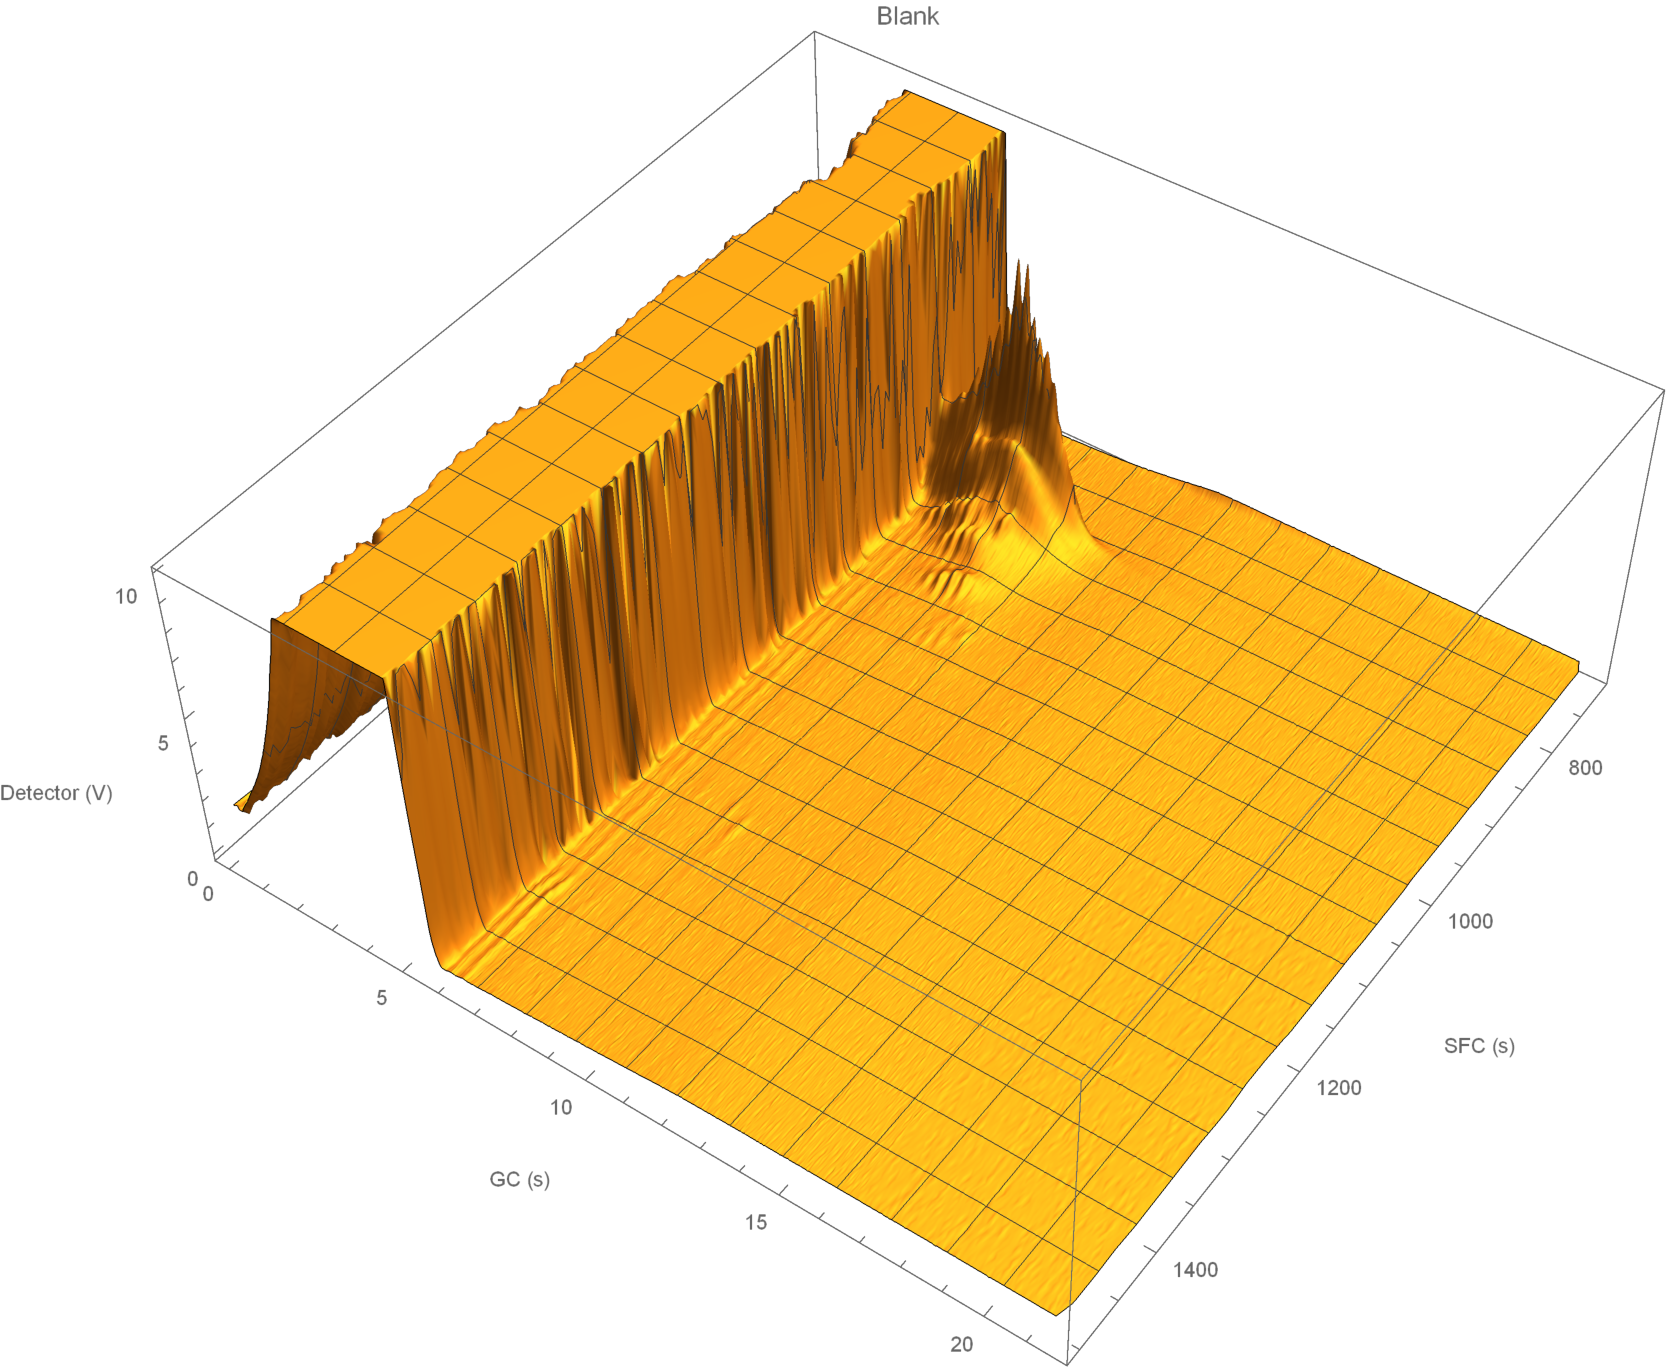
\includegraphics[width=\textwidth]{Figures/Modifier.pdf}
	\decoRule	
	
	\caption[Modifiers in SFC]{The modifier used in the SFC dimension elutes as a
solvent front on the GC dimension, and does not otherwise affect the separation.}
	
	\label{fig:Modifier} 
\end{figure}

The purpose of doing this chromatographic run was to explore the effect of the
methanol modifier on the retention behaviour of the biodiesel fraction of the
B50 blend. However, the run time was not long enough for the FAMEs to elute and
the only peaks on the chromatogram are the group of hydrocarbons from the
petrodiesel. Nevertheless, the chromatogram shows the possibilities that arise
when a modifier is added to the SFC mobile phase.

The 'wall' that appears on the chromatogram is the tailing edge of the peak of
the modifier added to the SFC. These peaks are present in all the fractions at
equal concentration. The flat top of the peak is caused by \keyword{detector
overload}. It should be emphasized that this overload is not caused by
saturation of the FID response, but by limits imposed by the chosen signal
amplifier. The FID has a dynamic range of 10\textsuperscript{6} and could
comfortably accommodate the modifier peak, but the amplifier gain was chosen to
best match the analyte signal with the input range of the 16-bit
analog-to-digital converter.

The 'corrugations' on the wall can be ascribed to two sources. Firstly, there
may be variations in retention time of the modifier peak, which can be caused by
variations in GC gas flow and variations in the fast temperature programs.
Second, variations in the amount of modifier collected by the modulator will
also cause slight changes in the apparent position of the peak. This second
reason is probably the major contributor for this run, caused by variations in
the timed collection period introduced by the imprecision of the
electromechanical valve actuator and by variations in the SFC flow.

The chromatogram shows the hydrocarbon ``hump'' in the GC dimension and the
separation of the aromatics in the SFC dimension, as discussed in Section
\ref{Chapter7}. It can be seen that the 'solvent peak' of the modifier
interferes with the more volatile of the hydrocarbons, but the rest of the
separation space is available for separation.

\subsection{Conclusion}

Adding modifiers to SFC expands the versatility of carbon dioxide as a mobile
phase, but in 1D SFC the use of modifiers precludes the use of the universal
flame ionization detector (FID), because the modifier signal will swamp the
analyte signal. Adding GC-FID as a \twoD separation allows the use of any
volatile modifier to manipulate retention in the SFC dimension, including
modifiers that might not be UV-transparent. Modifiers present in the fraction
collected by the modulator elute like the customary solvent peak in the GC
dimension, which means that the signal from the modifier does not interfere with
the signal of the analyte, if it is given that the analyte is less volatile than
the modifier.
 
The example above shows that SFC×GC will reliably separate methanol used as an
SFC modifier from the less-volatile analytes found in a biodiesel blend sample,
promising the use of FID as a detector for gradient-elution SFC×GC separations
of biodiesel and biodiesel blends.
